\subsection{Diagrama de Blocos}

O diagrama de blocos apresentado na Figura 1 ilustra a arquitetura geral do sistema, evidenciando os principais módulos e o fluxo de dados entre eles.

O sistema eletrônico opera com o microcontrolador ESP32 como núcleo central de processamento. O sensor DHT11 realiza as medições de temperatura e umidade, transmitindo os dados ao ESP32 via protocolo single-bus. O ESP32 processa as leituras e as disponibiliza na interface web por meio do módulo Wi-Fi integrado, utilizando o protocolo HTTP/HTTPS, sendo essa conectividade um requisito essencial para o envio dos dados ao banco de dados e à interface do cliente.

Os LEDs indicadores serão acionados diretamente pelos pinos digitais do ESP32, refletindo o modo de operação ativo. Quando um comando de alternância de modo é recebido via interface web, o firmware atualiza o estado interno e aciona o LED correspondente.\\

\begin{figure}[H]
   \centering
   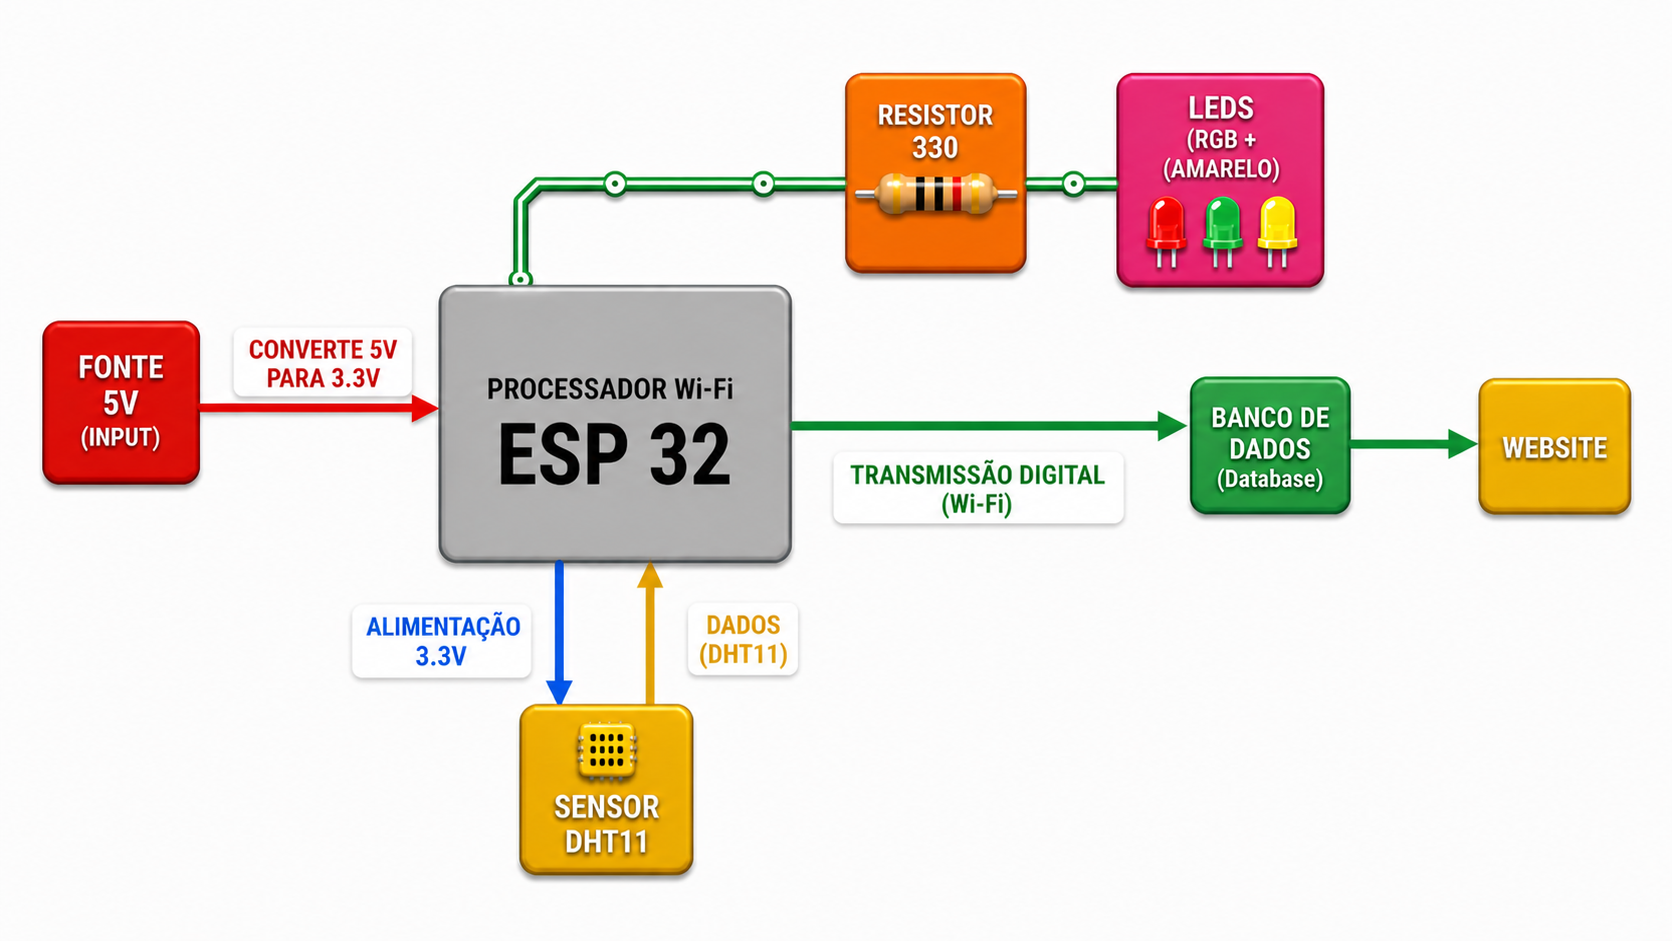
\includegraphics[width=0.7\textwidth]{imagens/diagramaemblocos.png} 
    \caption{Diagrama de blocos do sistema de monitoramento ambiental com ESP32 e DHT11.}
\end{figure}

\subsection{Esquemático Eletrônico}

%texto sobre o esquemático eletronico
As conexões do sensor DHT11 com a ESP32 são: VDD no 3.3V, DATA no pino 15 e GND no GND. Já as conexões dos LEDs com a ESP32 são: LED D1 no pino 32, LED D2 no pino 26, LED D3 no pino 12 no ânodo dos LEDs. No cátodo dos LEDs, todos estão interconectados e se ligam na trilha que vai para o GND da ESP32.

\begin{figure}[H]
   \centering
   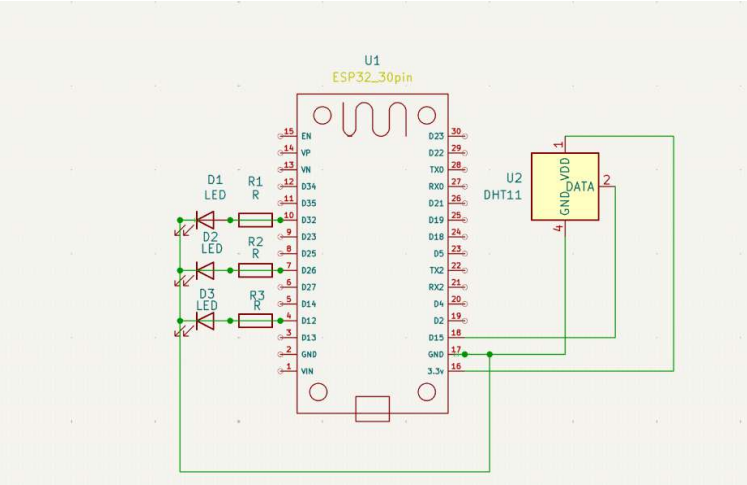
\includegraphics[width=0.7\textwidth]{imagens/esquemático.png} 
    \caption{Esquemático com ESP32 e DHT11.}
\end{figure}